% Author: Nikitha Jayant Bangera
% Version: 1.0

\documentclass[12pt, a4paper]{report}
\usepackage[left=2.5cm, right=2.5cm, top=1cm, bottom=1.5cm]{geometry}
\usepackage[utf8]{inputenc}
\usepackage{amssymb}
\usepackage{amsmath}
\usepackage{latexsym}
\usepackage[normalem]{ulem}
\usepackage{array}
\usepackage{graphicx, tabularx}
\usepackage[backend=biber,
style=numeric,
sorting=none,
isbn=false,
doi=false,
url=false,
]{biblatex}\addbibresource{bibliography.bib}
\usepackage{biblatex}
\usepackage{array,multirow}
\usepackage{longtable}

\date{}

\title{Eternity: Numbers}
\author{\\ \Large{Author Name}
\\ Nikitha Jayant Bangera
\\
\\
\\
\\ Concordia University
\\
A project report presented for the course\\ 
SOEN 6481 \\\textit{Software Requirements Specifications}
\\ \\ \\ \\
Under the guidance of\\
Professor Pankaj Kamthan
}
%%%%%%%%%%%%%%%%%%%%%%%%%%%%%%%%%%%%%%%%%%%%%%%%%%%%%%%%%%%%%%%%%%%%%%%
\begin{document}
\thispagestyle{headings}
	\maketitle
\pagenumbering{roman}

\thispagestyle{empty}
\chapter*{Acknowledgements}
I would like to express my sincere thanks to Professor Pankaj Kamthan for his advice and encouragement throughout the First deliverable of the Eternity: Numbers project, as well as to my Technical Lab Assistant for his guidance throughout the first phase of the project. 
\thispagestyle{empty}
\begin{abstract}
%\lipsum[1-2]
The document tries to put some light on the understanding of an irrational number, The Champernowne Constant. A brief description of the constant and some of its applications are included in the report. A research and interview on the constant was conducted with a resource who is familiar with Champernowne constant. My interviewee tried to answer most common questions about the constant in a questionnaire that also describes some applications of Champernowne constant. Based on the understanding of Champernowne Constant, a calculator application is to be built, that uses this constant to perform certain operations. This document also gives the basic design details on how the product would look like,what operations is it capable of, its algorithm and use cases.
\end{abstract}

\tableofcontents
\thispagestyle{plain}
\listoffigures
\listoftables

\chapter{Introduction}
\pagenumbering{arabic}
\section{Champernowne's Constant Definition}
\quad Champernowne Constant is a real number whose decimal digits are obtained by concatenating the decimal expansions of the successive positive integers:\\\\
\hspace*{30mm} $C_{10}$ = 0.12345678910111213141516…\\\\
It is named after economist and mathematician David G. Champernowne, who published it as an undergraduate in 1933.\\
\section{Champernowne Constant as an Infinite series}
\quad The Champernowne constants can be expressed exactly as infinite series:\\\\
\hspace*{30mm} $\displaystyle C_m = \sum_{n=1}^{\infty} \frac{n}{{10_b}^{\displaystyle (\sum_{k=1}^n \lceil {log_{10}}_b (k+1) \rceil)}}$\\\\
where $\lceil x \rceil $ = ceiling(x), ${10_b}^x = b^x$ in base 10, ${log_{10}}_b (x) = {log_b}_{10} (x)$ and {\it b} is the base of the constant.\\
\section{Continued Fraction Expansion}
\quad The Continued Fraction Expansion (CFE) of the Champernowne constant turns out to be a set large numbers with various spikes. Kurt Mahler showed that the constant is transcendental; therefore, its continued fraction does not terminate and is aperiodic (because it is not an irreducible quadratic). The terms in the continued fraction expansion exhibit very erratic behaviour, with extremely large terms appearing between many small ones. The CFE begins with 0; 8, 9, 1, 149083, 1, 1, 1, 4, 1, 1, 1, 3, 4, 1, 1, 1, 15, and the coefficient in position 18 has 166 digits. The large number at position 18 has 166 digits, and the next very large number at position 40 of the continued fraction has 2504 digits. The fact that there are such large numbers as terms of the continued fraction expansion is equivalent to saying that the convergents obtained by stopping before these large numbers provide an exceptionally good approximation of the Champernowne constant.\\\\

\begin{figure}
    \centering
    \fbox{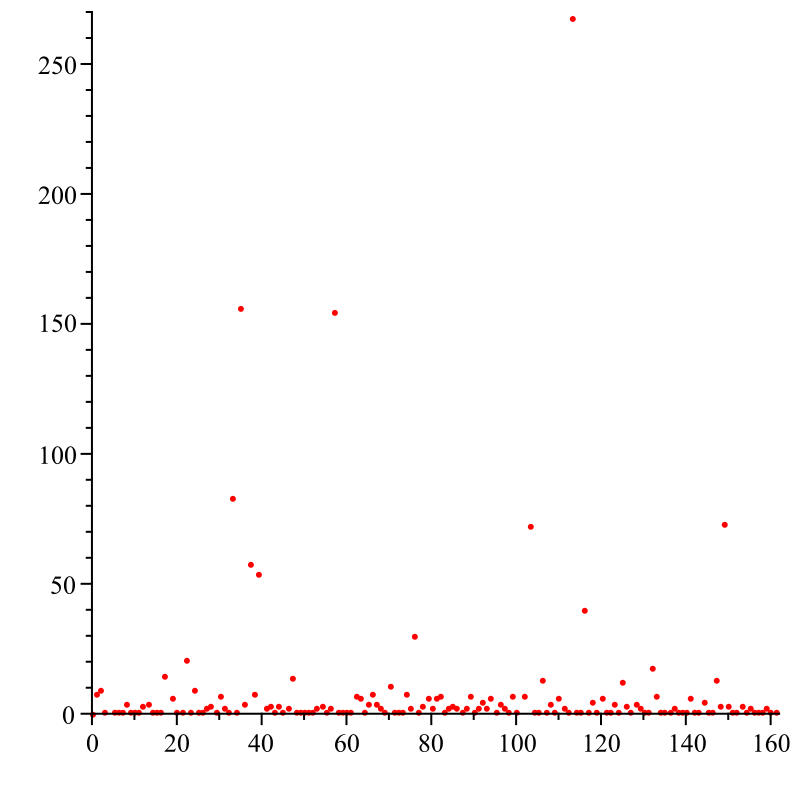
\includegraphics[width=100mm]{Champernowne_Constant.png}}
    \caption{The first 161 quotients of the Champernowne constant.}
    \label{fig:The first 161 quotients of the Champernowne constant.}
\end{figure}

\chapter{Interview}
\label{Chap2}
\section{Brief introduction about the Interviewee}
{\bf Name} : Megha Kamath \\
{\bf Qualification} : Masters in Mathematics \\
{\bf Reason behind opting the interviewee} : My Interviewee is pursuing Masters in Mathematics and it was obvious for me to work with her to better understand about the Champernowne constant and its applications.
\section{Interview Questions on Champernowne Constant}
\begin{enumerate}
	\item Could you mention some areas where Champernowne constant can be applied?
	\\ {\it The Champernowne constant has seemingly random numbers which are clearly well determined. This property could be useful in functional programming contexts where one would need explicit randomness which is entirely deterministic. For example, the C2 (Base 2) value of the Champernowne constant can be used as a binary random number to trigger true or false conditions randomly.}
	\item Could you mention the properties of the Champernowne constant?
	\begin{enumerate}
	{\it \item The constant given by 0.123456789101112 . . . is normal in base ten.
	\item The constant is transcendental.
	\item The constant also has a peculiar continued fraction expansion. It namely contains exceptionally large terms throughout the expansion.}
	\end{enumerate}
	\item Is Champernowne constant a Liouville number?
	\\ {\it No. Champernowne constant and Liouville numbers are both transcendental but Champernowne constant is irrational and Liouville numbers are almost rational and can be approximated quite closely by sequences of rational numbers than any algebraic irrational numbers.}
	\item Is Champernowne constant as useful as  \( \pi \) constant?
	\\ {\it The Champernowne constant is quite useful. But Pi is a constant which is there almost everywhere in mathematics. }
	\item Does it appear in any sort of geometric solutions like  \( \pi \) does?
	\\ {\it The Champernowne constant cannot be represented as a finite number due to which there have been no reported utilization in geometry.}
	\item How often do you use the Champernowne constant?
	\\ {\it As a student of pure mathematics I do not use the Champernowne constant quite often.}
	\item Has the Champernowne constant ever been used in any major proofs? 
	\\ {\it No.}
	\item Can it be expressed in terms of e,  \( \pi \) or both? 
	\\ {\it No.}
	\item What works of Alan Turing and David Champernowne made use of the Champernowne constant?
	\\ {\it Notably, There were two major works of Alan Turing and David Champernowne, the TuroChamp and Round the house Chess. But the Champernowne constant is not mentioned to have been in any of these machines.}
	\item Of all the base versions of Champernowne constants which particular Champernowne sequence has been vastly used?
	\\{\it Base 2 (C\textsubscript{2}) and Base 10 (C\textsubscript{10}).}
	\item Who and How was Champernowne constant proved Transcendental? 
	\\ {\it The Champernowne constant was shown to be transcendental by Kurt Mahler in 1937.}
	\item What are the alternatives available for Champernowne constant?
	\\ {\it None.}
	\item Is Champernowne constant used in Turochamp or Round the house Chess? if Yes, how does it fit into the algorithms of these games?
	\\ {\it No. }
	\item Do you think of any problem where Champernowne Constant would be a perfect fit to be used?
	\\ {\it I can actually think of 2, One being a Random Binary digit generator where Champernowne Constant of Base 2 would be a perfect fit and Two, Given a sequence of numbers (to base 10), How to calculate the position of any random number. I think Champernowne constant fits well into these scenarios. }
\end{enumerate}
\section{Analysis of the Interview}
\quad The Interviewee had moderate knowledge about the Champernowne constant. She was able to explain the basic characteristics of the constant with logical examples (mentioned in the response to the interview questions). The practical applications of the constant have been limited and the interviewee was able to explain one particular area where the constant (its base 2 value) is widely used to generate the randomized binary numbers.

\chapter{User model: Persona Template}
\begin{center}
\begin{tabular}{ | m{40em} | } 
\hline
\\\textbf{Private Information} \\
\begin{minipage}{0.70\textwidth}
\begin{itemize}
    \setlength{\itemsep}{0pt}
    \item Name: Megha Kamath
    \item Qualification: Currently pursuing Masters in Mathematics
    \item University: Mangalore University, Karnataka, India
    \item Megha lives in Karnataka, India with her parents.
    \item She loves to read fictional novels and also cooking is her favourite pass-time.
\end{itemize}
\end{minipage}
\begin{minipage}{0.3\textwidth}
\fbox{
\includegraphics[width=\linewidth, height=4cm]{student.jpg}}
\end{minipage}
\\
\hline
\\\textbf{Use of Number, relation to Number} \\
Based on the conversation with interviewee -\\
\begin{itemize}
    \setlength{\itemsep}{0pt}
    \item The Champernowne constant has seemingly random numbers which are clearly well determined. This property could be useful in functional programming contexts where one would need explicit randomness which is entirely deterministic.
    \item  Base 2 of the Champernowne constant is in functional programming as a Random Binary Digit Generator.
\end{itemize}
\\
\hline
\\\textbf{Description of work or daily life} \\
\begin{itemize}
    \setlength{\itemsep}{0pt}
    \item Megha is in her First Year of Masters in Mathematics. Her specialization is Pure Mathematics.
    \item She has moderate knowledge about the Champernowne Constant.
    \item She does not use the Champernowne constant quite often as her specialization is Pure Mathematics.
\end{itemize}
\\
\hline

\end{tabular}
\begin{tabular}{ | m{40em} | }
\hline
\\\textbf{Other uses or relations to the Number} \\
\begin{itemize}
     \setlength{\itemsep}{0pt}
    \item As per Megha's research, the Champernowne constant was never used in major proofs.
    \item Due to the constant's inefficient nature, the constant is mostly avoided in mathematical calculations.
\end{itemize}
\\
\hline
\\\textbf{Influencers that surround the persona and that may influence choices}\\
\begin{itemize}
    \setlength{\itemsep}{0pt}
    \item Professors
    \item Friends
    \item Classmates
\end{itemize}
\\
\hline
\end{tabular}
\end{center}

\chapter{Problem Domain Model}
\section{UML Class Diagram}
Figure 4.1 shows the Class diagram of the Eternity: Numbers system which shows the different concepts, properties of each concepts and the relationship between the concepts
\begin{figure}
    \centering
    \fbox{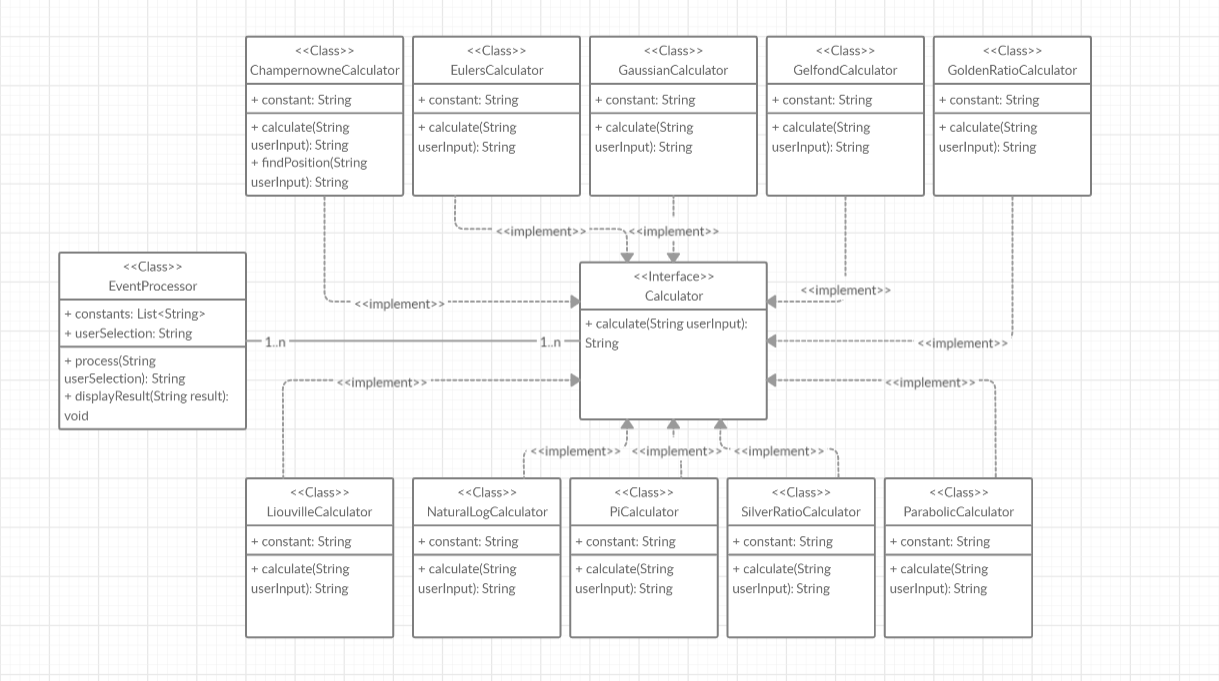
\includegraphics[width=160mm,height=100mm]{CalculatorClassDiagram.PNG}}
    \caption{UML Class Diagram of Eternity: Numbers}
    \label{fig:UML Class Diagram of Eternity: Numbers}
\end{figure}

\begin{itemize}
    \item \textbf{Interface: Calculator.java:} Interface class that defines the calculate method signature for which is implemented by the classes that perform operations on the Eternity: Numbers.
    \item \textbf{Class: EventProcessor.java:} Is the main class of the calculator. It is the starting point of the product, Eternity: Numbers and it does the following operations:
    \begin{itemize}
        \item Allows user to pick a constant to perform calculations,
        \item Invokes the relevant calculator class to process user requests and
        \item Display the processed/calculated result to user.
    \end{itemize}
    \item \textbf{Class: EulersCalculator.java:} This class performs key operations on Euler’s constant. Since our focus is more on the Champernowne constant. This class is designed to request user to choose Champernowne constant from the startup menu.
    \item \textbf{Class: GaussianCalculator.java:} This class performs key operations on Gaussian Integral constant. Since our focus is more on the Champernowne constant. This class is designed to request user to choose Champernowne constant from the startup menu.
    \item \textbf{Class: GelfondCalculator.java:} This class performs key operations on Gelfond’s constant. Since our focus is more on the Champernowne constant. This class is designed to request user to choose Champernowne constant from the startup menu.
    \item \textbf{Class: GoldenRatioCalculator.java:} This class performs key operations on Golden Ratio. Since our focus is more on the Champernowne constant. This class is designed to request user to choose Champernowne constant from the startup menu.
    \item \textbf{Class: LiouvilleCalculator.java:} This class performs key operations on Liouville constant. Since our focus is more on the Champernowne constant. This class is designed to request user to choose Champernowne constant from the startup menu.
    \item \textbf{Class: NaturalLogCalculator.java:} This class performs key operations on Natural Logarithm. Since our focus is more on the Champernowne constant. This class is designed to request user to choose Champernowne constant from the startup menu.
    \item \textbf{Class: PiCalculator.java:} This class performs key operations on Pi constant. Since our focus is more on the Champernowne constant. This class is designed to request user to choose Champernowne constant from the startup menu.
    \item \textbf{Class: SilverRatioCalculator.java:} This class performs key operations on Silver Ratio. Since our focus is more on the Champernowne constant. This class is designed to request user to choose Champernowne constant from the startup menu.
    \item \textbf{Class: ParabolicCalculator.java:} This class performs key operations on Universal Parabolic constant. Since our focus is more on the Champernowne constant. This class is designed to request user to choose Champernowne constant from the startup menu.

\end{itemize}

\chapter{Use Case Model}
\section{UML Use Case Diagram}
\begin{figure}
    \centering
    \fbox{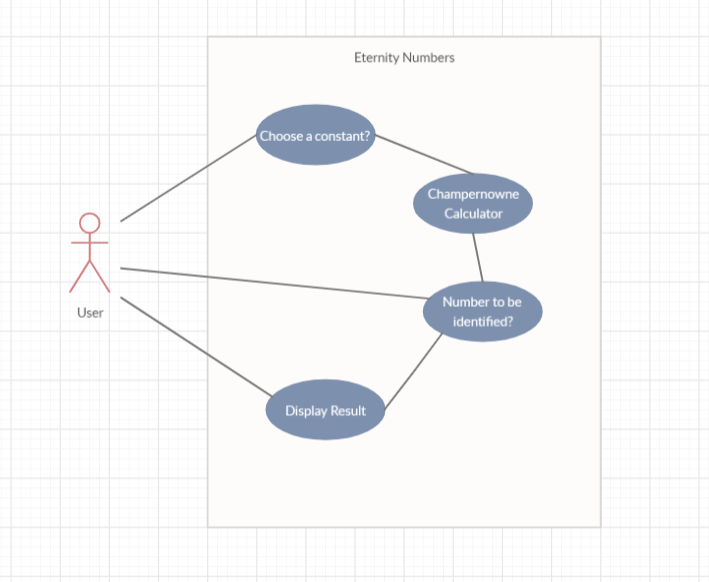
\includegraphics[width=160mm]{ChampernowneUseCase.PNG}}
    \caption{UC001 - UML Use Case diagram of Eternity: Numbers}
    \label{fig:UML Use Case diagram of Eternity: Numbers}
\end{figure}
Steps in the Use case model of Eternity numbers calculator (Refer to Figure 5.1):
\begin{enumerate}

    \item User starts the calculator application i.e. Eternity: Numbers constant. The application displays a set of constants(Eternity: Numbers), which a user can pick to perform various operations.
    \item User selects the Champernowne Constant.
    \item The applications prompts the user to enter any random number between 0 and 180000, for which the user would want to know the position in the Champernowne constant.
    \item User enters the number.
    \item The system processes user's input and displays the position of the number given by the user.
\end{enumerate}
\section{UML Activity Diagram}
Figure 5.2 shows the Activity diagram representation of the above use case. If the user selects any other constant other than the Champernowne constant, a relevant message is displayed that the feature is not available as this version of the product focuses on Champernowne Constant only.\\\\
%\hspace{15mm}
\begin{figure}
    \centering
    \fbox{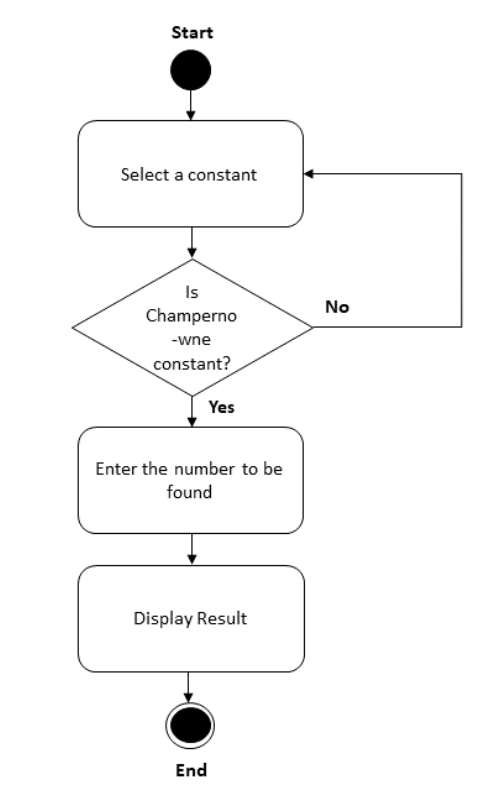
\includegraphics[width=100mm, height=140mm]{ChampernowneActivity.PNG}}
    \caption{UML Activity diagram of Eternity: Numbers}
    \label{fig:UML Activity diagram of Eternity: Numbers}
\end{figure}
\section{Normal Scenario of Use case model}
Figure 5.3 shows the normal scenario in the use case model of the Eternity Numbers application
\begin{figure}
    \centering
    \fbox{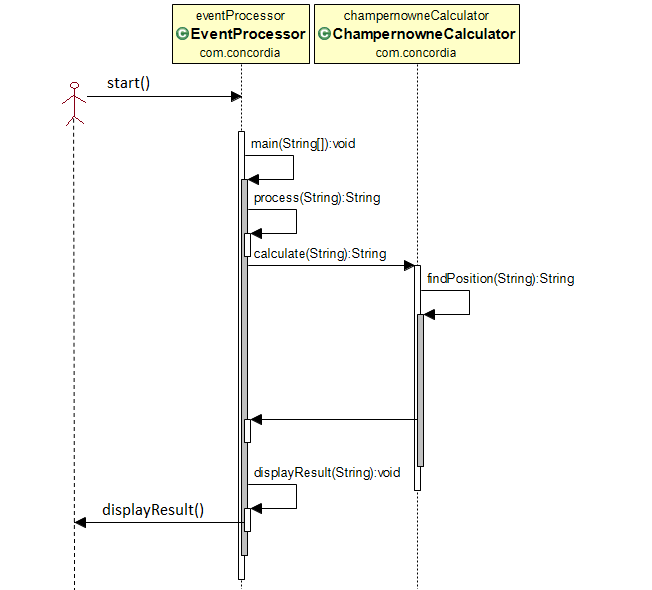
\includegraphics[width=150mm, height=140mm]{EternityNumbersSequenceDiagram.png}}
    \caption{UML Sequence diagram of Eternity: Numbers}
    \label{fig:UML Sequence diagram of Eternity: Numbers}
\end{figure}
\chapter{User stories and Traceability Matrix}
\section{User stories and Acceptance Test cases}
The following table describes the list of user stories and acceptance test cases for every user story.
\\
\begin{longtable}{|p{1cm}|p{8em}|p{2em}|p{2em}|p{1cm}|p{3cm}|p{4.5cm}|}
\hline
     \multicolumn{2}{|c|}{\textbf{User stories}} & \multicolumn{2}{|c|}{} & \multicolumn{3}{|c|}{\textbf{Acceptance Test Cases}}  \\
     \hline
     Story ID & Story Description & Prio-rity & Esti-mate & Test Case ID & Test Case Description & Test Case Output\\\hline
     \multirow{3}{}{US001} & \multirow{3}{8em}{As a user, I want to have a calculator application that helps me with calculations using irrational numbers like Champernowne Constant, Guassian Integral, Pi etc. The application should let me choose the constant I want to use in my calculations and prompt me with options the calculator is capable of doing for a Chosen constant.} & \multirow{3}{}{1} & \multirow{3}{}{1} & TC001 & Start the calculator application. Select 1 for Champernowne Constant. & The application should display all the constants which a user can choose to perform required actions.The application should display a question, Choose the type of number(Binary or Integer) to find its position.\\\cline{5-7}
     & & & & TC002 & Start the calculator application. Select 20 for an unknown Constant. & The application should display all the constants which a user can choose to perform required actions. The application should display a message, "Please make a valid selection".\\\cline{5-7}
     & & & & TC003 & Start the calculator application. Select 2 for Eulers constant. & The application should display all the constants which a user can choose to perform required actions. The application should display a message, "The application is designed only for Champernowne Constant, please choose accordingly".\\\hline
     \multirow{3}{}{US002} & \multirow{3}{8em}{As a user, I want to identify a position of binary and integer numbers in a sequence of incremental positive numbers. For this I want a calculator application, that will allow me to input my choice of type of number (Binary or Integer) for which I want to calculate the position for, based on my selection, I want the app to ask for entering a number and display the position of that number.} & \multirow{3}{}{2} & \multirow{3}{}{2} & TC004 & Start the calculator application. Select 1 for Champernowne Constant. Select 1 for type of number. & The application should display all the constants which a user can choose to perform required actions.The application should display a question, Choose the type of number(Binary or Integer) to find its position. The application should display a question, "Enter a number to find its position".\\\cline{5-7}
     & & & & TC005 & Start the Calculator application. Select 1 for Champernowne Constant. Select 3 for type of number. & The application should display all the constants which a user can choose to perform required actions.The application should display a question, "Choose the type of number(Binary or Integer)" to find its position. The application should display a message, "Incorrect selection, please choose 1 for Binary or 2 for Integer".\\\cline{5-7}
     & & & &TC006&Start the Calculator application. Select 1 for Champernowne Constant. Select 2 for type of number. & The application should display all the constants which a user can choose to perform required actions.The application should display a question, "Choose the type of number(Binary or Integer)" to find its position.The application should display a question, "Enter a number to find its position".\\\hline
     \multirow{3}{}{US003} & \multirow{3}{8em}{As a user, I want to have a calculator application that can help me find the position of a binary equivalent of a Positive integer. For this, I want the calculator application to let me input the binary number of my choice and display the natural position of the binary number in the sequence of incremental positive binary numbers.} & \multirow{3}{}{3} & \multirow{3}{}{4} & TC007 & Start the calculator application. Select 1 for Champernowne Constant. Select 1 for type of number. Enter 100 as the number to find its position. & The application should display all the constants which a user can choose to perform required actions. The application should display a question, "Choose the type of number(Binary or Integer)" to find its position. The application should display a question, "Enter a number to find its position". The application should display the message, "The position of number 100 in Base 2 of Champernowne constant is 5".\\\cline{5-7}
     & & & & TC008 & Start the calculator application. Select 1 for Champernowne Constant. Select 1 for type of number. Enter 123 as the number to find its position. & The application should display all the constants which a user can choose to perform required actions.The application should display a question, "Choose the type of number(Binary or Integer)" to find its position. The application should display a question, "Enter a number to find its position". The application should display the message, "Please enter a valid binary number".\\\cline{5-7}
     & & & & TC009 & Start the calculator application. Select 1 for Champernowne Constant. Select 1 for type of number. Enter 0.100 as the number to find its position. & The application should display all the constants which a user can choose to perform required actions.The application should display a question, "Choose the type of number(Binary or Integer)" to find its position. The application should display a question, "Enter a number to find its position". The application should display the message, "Please enter a valid binary number".\\\hline
     \multirow{3}{}{US004} & \multirow{3}{8em}{As a user, I want to find the starting position of a given number in a sequence of positive integers. For this, I would want a calculator application that will allow me to input a number of my choice and display the natural position of the number in an incremental sequence of positive integers.} & \multirow{3}{}{3} & \multirow{3}{}{4} & TC010 & Start the calculator application. Select 1 for Champernowne Constant. Select 2 for type of number. Enter 100 as the number to find its position. & The application should display all the constants which a user can choose to perform required actions. The application should display a question, "Choose the type of number(Binary or Integer)" to find its position. The application should display a question, "Enter a number to find its position". The application should display the message, "The position of number 100 in Base 10 of Champernowne constant is 210".\\\cline{5-7}
     & & & & TC011 & Start the calculator application. Select 1 for Champernowne Constant.Select 2 for type of number. Enter 104 as the number to find its position. & The application should display all the constants which a user can choose to perform required actions. The application should display a question, "Choose the type of number(Binary or Integer)" to find its position. The application should display a question, "Enter a number to find its position" .The application should display the message, "The position of number 100 in Base 10 of Champernowne constant is 222".\\\cline{5-7}
     & & & & TC012 & Start the calculator application. Select 1 for Champernowne Constant. Select 2 for type of number. Enter -11000000 as the number to find its position. & The application should display all the constants which a user can choose to perform required actions. The application should display a question, "Choose the type of number(Binary or Integer)" to find its position. The application should display a question, "Enter a number to find its position" .The application should display the output , "Please enter a valid Positive integer number".\\\hline
\caption{Table of User stories and Acceptance Test cases}
\label{table:1}
\end{longtable}

\section{Backward Traceability Matrix}

\begin{longtable}{|p{2.5cm}|p{2cm}|p{2cm}|p{2cm}|p{4cm}|}

    \hline
    \textbf{User Stories} & \textbf{Test Cases} & \textbf{Use Case} & \textbf{Persona} & \textbf{Requirements/ Interview Questions} \\\hline
   \multirow{3}{0pt}{US001} & TC001 & UC001 & Interviewee & 1,2 \\\cline{2-5}
   & TC002 & UC001 & Developer & 1,2 \\\cline{2-5}
   & TC003 & UC001  & Developer & 1,2 \\\hline
   \multirow{3}{}{US002} & TC004 & UC001 & Interviewee & 10 \\\cline{2-5}
   & TC005 & UC001 & Interviewee & 10 \\\cline{2-5}
   & TC006 & UC001 & Developer & 10 \\\hline
   \multirow{3}{}{US003} & TC007 & UC001  & Interviewee & 10,14 \\\cline{2-5}
   & TC008 & UC001 & Developer & 10,14 \\\cline{2-5}
   & TC009 & UC001 & Developer & 10,14 \\\hline
   \multirow{3}{}{US004} & TC010 & UC001  & Interviewee & 10,14 \\\cline{2-5}
   & TC011 & UC001 & Developer & 10,14 \\\cline{2-5}
   & TC012 & UC001 & Developer & 10,14 \\\hline
\caption{Table for Backward Traceability Matrix}
\label{table:1}
\end{longtable}
{*Refer Figure 6.1 for the User Stories and Figure 5.1 for the Use Case Diagram.}

\begin{thebibliography}{9}
    \bibitem {Wikipedia}
    \texttt{https://en.wikipedia.org/wiki/Champernowne{\_}constant}
    \bibitem {Wolfram}
    \texttt{http://mathworld.wolfram.com/ChampernowneConstant.html}
    \bibitem{wikia}
    \texttt{https://googology.wikia.org/wiki/Champernowne{\_}constant{\_}continued{\_}fraction}
    \bibitem {FSE}
    \texttt{http://fse.studenttheses.ub.rug.nl/}
    \bibitem {Online Encyclopedia Champernowne constant base 10}
    \texttt{https://oeis.org/A065649}
\end{thebibliography}
\end{document}
